\documentclass[11pt, a4paper]{article}
\usepackage[utf8]{inputenc}
\usepackage{mathpazo} % Palatino font
\usepackage{lineno}
\usepackage{setspace}
\usepackage{caption}
\usepackage{graphicx, subfig}
\usepackage{cite}
\usepackage{float} %so the graphs are not floating around after I put[H]
\usepackage[margin=2cm]{geometry}
\usepackage{indentfirst}
\usepackage{natbib} 

\begin{document}
\begin{spacing}{1.5}

\begin{titlepage} % Suppresses displaying the page number on the title page and the subsequent page counts as page 1
	\newcommand{\HRule}{\rule{\linewidth}{0.5mm}} % Defines a new command for horizontal lines, change thickness here
	
	\center % Centre everything on the page
	
	%------------------------------------------------
	%	Headings
	%------------------------------------------------
	
	\textsc{\LARGE Imperial College London}\\[2.5cm] % Main heading such as the name of your university/college
	
	\textsc{\Large Computational Method in Ecology and Evolution}\\[2.5cm] % Major heading such as course name
	

	%------------------------------------------------
	%	Title
	%------------------------------------------------
	
	\HRule\\[0.6cm]
	
	{\huge\bfseries Thermal Response Model Selection and Analysis is Dependent on the Studied Traits and Temperature Range}\\[0.4cm] % Title of your document
	
	\HRule\\[2.5cm]
	
	%------------------------------------------------
	%	Author(s)
	%------------------------------------------------
	
	\begin{minipage}{0.4\textwidth}
		\begin{center}
			\large
			\textit{Author: }
			\text{Danica Duan}\\
			\textit{CID: }
			\text{01790819}% Your name
		\end{center}
	\end{minipage}

	
	% If you don't want a supervisor, uncomment the two lines below and comment the code above
	%{\large\textit{Author}}\\
	%John \textsc{Smith} % Your name
	
	%------------------------------------------------
	%	Date
	%------------------------------------------------
	
	\vfill\vfill\vfill % Position the date 3/4 down the remaining page
	
	{\large\today} % Date, change the \today to a set date if you want to be precise

	 
	%----------------------------------------------------------------------------------------
	
	\vfill % Push the date up 1/4 of the remaining page
	Word Count: 2378

\end{titlepage}

%----------------------------------------------------------------------------------------



\section*{Abstract}
Understanding thermal responses of metabolic rate is fundamental for studying the impacts of changing temperature from cellular level to the ecosystem. Among a wide range of published models, I fitted 3 phenomenological (cubic, quadratic and Briere) and 1 mechanistic (simplified Schoolfield) model in this project to a subset of bio-trait data. After model selection and comparison, the linear cubic model provides best simulation for temperature response of respiration, given most data collected under regular environmental temperature does not reach the optimum rate temperature for respiration; and the Schoolfield model provides best simulation for photosynthesis. Through parameter estimations of the Schoolfield model, the respiration shows higher sensitivity to high temperature than respiration, and the activation energy for metabolism of aquatic organism is significantly higher than that for terrestrial organisms.  

\linenumbers
\renewcommand\thesection{\arabic{section}}
\section{Introduction}

Since temperature is one of the major factors direct or indirectly affecting a wide range of biological rates, from biochemical reaction in cells to functions of the ecosystem \citep{brown2004toward, schulte2015effects}. Understanding thermal responses of metabolic rate is fundamental for studying the impacts of changing temperature on major bioprocesses such as growth, respiration, and photosynthesis. 

Chemical reaction rates are known to increase with rising temperature. According to the dominant theory of chemical kinetics --- the Arrhenius equation \citep{menzinger1969meaning}, the relationship of reaction rate with temperature is governed by the energy barrier for molecule activation known as the activation energy (Ea) and the collision frequency of the activated molecules (A), which are both assumed to be independent of temperature. $k(T)= Ae^{-E_a/kT}$ is the equivalent version of the original Arrhenius equation, in which k(T) is the reaction rate, T is temperature (K), and k is the Boltzmann constant ($8.617\times10^{-5}eV\cdot K^{-1}$).

However, bioprocesses are dominated by enzyme reactions which only operates under optimal temperature range and denatures at a certain high and low temperature, therefore cannot be properly described by Arrhenius equation. Hence various mechanistic models have been proposed to describe the unimodal response of multiple bioprocesses with a wider range of temperature \citep{johnson1946growth, rezende2019thermal, schoolfield1981non}, and to test and understand the underlying mechanistic theory of thermal performance among different metabolism, taxa, habitat, etc. \citep{dell2011systematic} through predicting the activation energies and optimal temperature for metabolic rates. These estimations could vary significantly with habitats due to adaptation \citep{sage2007temperature}; and traits, due to the entirely different pathways and reactions within those two metabolisms \citep{raven2005biology, ABEDON20083010}.

In addition to mechanistic models, phenomenological models \citep{ratkowsky1983model, boatman2017key, briere1999novel} were also widely developed to simulate the unimodal temperature response of bio-traits, which includes applying quadratic, Gaussian and modified Gaussian equations to empirical data \citep{montagnes2008short}. 

The aim of this project is to compare and determine the suitability of these models to a subset of field and lab collected data. Research questions are: 1) Are non-linear model better for simulating the thermal responses of the dataset? 2) Is the mechanistic model suitable for simulating this dataset? 3) Do estimated parameter values from the mechanistic model differ with metabolic rates/habitats?   

\section{Methods}

\subsection{Data and Model Fitting}

The given dataset is a subset of the “BioTraits” database, containing thermal responses of respiration and photosynthesis rates (net photosynthesis = gross photosynthesis - respiration) in different taxa of plant and bacteria from different habitats across the world. The trait values collected were calculated as the difference of measured with the reference data. 

I first discarded all negative trait values, since negative metabolic rates of respiration and photosynthesis are not possible under real-life scenario. Then I applied two linear phenomenological models --- quadratic and cubic equations, and two non-linear models the Briere model (phenomenological) and the Schoolfield model (mechanistic). 

Since R has more statistic and graphing packages and is more well-used in data analysis, I used R for conducing this project. Function lm was used for fitting linear models and function nlsLM from package minpack.lm \citep{elzhov2016package} was used for fitting non-linear models. 

The Briere model \citep{briere1999novel} was developed aiming at reducing parameters in describing the non-linear relationship of traits to temperature. \begin{equation}
    B = \left\{
    \begin{array}{cc}
        0 & T \leq T0 \\
        B_0T(T - T_0)\sqrt{T_m - T} & T_0 \leq T \geq T_m \\
        0 & T \geq Tm
    \end{array}\right.
\end{equation}
In this equation, B represents the trait (such as growth, respiration or photosynthesis) value at given temperature, $B_0$ is the normalization constant and $T_0$ and $T_m$ are the minimum and maximum feasible temperatures for the trait.

I used maximum and minimum temperature values of each data subset at each sample ID as their $T_m$ and $T_0$ starting values. And I obtained starting $B_0$ values for the Briere model by: 1) input the trait values of data subsets of each sample ID into the Briere model equation; 2) then calculate the mean value of all $B_0$ values obtained; 3) use this value as the mean value for a normal distribution with the absolute mean value for the standard deviation (since the differences of trait values are of magnitudes among samples), and sample the starting $B_0$ value from this normal distribution. 

Since the $T_m$ and $T_0$ values are the maximum and minimum feasible temperature, a wide enough boundary range is given to prevent good but biologically meaningless fits of the model. For the Briere model, I chose -80-40 $^{\circ}$C for $T_0$ and 0-100 $^{\circ}$C for $T_m$. 

The Schoolfield model \citep{schoolfield1981non}:  
\begin{equation}
    B = \frac{B_0e^{-\frac{Ea}{k}(\frac{1}{T} - \frac{1}{283.15})}}{1+e^{\frac{E_l}{k}(\frac{1}{T_l} - \frac{1}{T})}+e^{\frac{E_h}{k}(\frac{1}{T_h} - \frac{1}{T})}}
\end{equation}
In this equation, $B_0$ is the trait value at reference temperature, $E_l$ and $E_h$ are the low- and high-temperature deactivation energy, $T_l$ and $T_h$ are the low- and high- temperature at which the enzyme is 50\% deactivated. 

I applied the simplified version of Schoolfield model without low temperature deactivation since the data from low temperature is not sufficient. 
\begin{equation}
    B = \frac{B_0e^{-\frac{Ea}{k}(\frac{1}{T} - \frac{1}{283.15})}}{1+e^{\frac{E_h}{k}(\frac{1}{T_h} - \frac{1}{T})}}
\end{equation}

The starting values of Ea and Eh for fitting the Schoolfield model were obtained from linear fitting of the log transformed version of Arrhenius equation with data subsets of before (for Ea) and after (for Eh) high temperature deactivation. Considering the trait values were collected by comparing to a reference value at a reference temperature of 10 $^{\circ}$C, the log version of Arrhenius equation should be transformed as follow: 
\begin{equation}
    lnk(T)= ln{B_0}-\frac{E}{kT}
\end{equation}
\begin{equation}
    \int_{T_{ref}}^T \frac{dlnk(T)}{dT}=\frac{E}{kT^2}
\end{equation}
Therefore getting (k(T) as B and $T_{ref}$ as 283.15 K):
\begin{equation}
    lnB = -\frac{E}{k}(\frac{1}{T}-\frac{1}{283.15})+lnB_0
\end{equation}
By fitting this equation with lnB value and ($-\frac{1}{kT}+\frac{1}{283.15}$), then getting the slope and intercept values, I got the starting values of both E and $lnB_{0}$. 

Bounds were selected to be slightly wider than reported normal ranges for activation/deactivation energies and temperature at maximum metabolic rates to eliminate biologically meaningless fittings \citep{gillooly2001effects, zwietering1991modeling, doran1995homogeneous}, as 273-333 K (0-60 $^{\circ}$C) for $T_h$, 0-2 eV for $E_a$, and 0-5 eV for $E_h$. 

\subsection{Model Assessment}
I applied Akaike information criterion (AIC) and Bayesian information criterion (BIC) as selection criteria for model assessment \citep{johnson2004model}, among which BIC tends to favor simpler models with a punishment for model complexity in the calculation equation (as below). Small sample unbiased AIC (AICc) was inefficient due to the low sample size ($n \le 5$) of large number of curves. The calculation equations are shown below, with $ln[L(\hat{\theta}_y]=-n/2ln(RSS/n)$ for least squares model fits. 
\begin{equation}
    AIC = -2ln[L(\hat{\theta}_y]+2p
\end{equation}
\begin{equation}
    BIC = -2ln[L(\hat{\theta}_y]+p\cdot ln(n)
\end{equation}

The performance of different models to data are evaluated with delta AIC and delta BIC methods, which is calculating the difference between candidate AIC (BIC) with the minimum AIC (BIC) values (the best fit). Since the lower AIC (BIC) the better, in this method, if the difference is less than 2, then it provides substantial evidence for the candidate model to be well supported by the data as well \citep{burnham2002practical, raftery1995bayesian}. 

\subsection{Statistical Analysis of Model Prediction}

Activation and deactivation energies, and the temperatures of maximum metabolic rates for the thermal response curves are estimated by fitting the Schoolfield model equation to the given data. These estimations were further tested by ANOVA (with pairwise t-test) and t-test to analyse the mean value and significance of differences among different habitats and between respiration and photosynthesis. 

\section{Results}

Out of all 903 sample sets, 897 remained after discarding all negative metabolic rates of the data subset, 98.2\% among which have more than 5 data points. 74.0\% of temperature response data are unimodal shaped with a maximum temperature and decreasing rate values after high temperature deactivation, most of the rest are singularly increasing without reaching the half deactivation temperature, several has higher temperature sensitivity thus the metabolic rates were falling right from the start of the measurements. 

A good example for simulation of all four models (quadratic, cubic, Briere and Schoolfield) to a unimodal temperature response curve of net photosynthesis rate (sample ID: 341, the shoots stage of a freshwater aquarium plant species \textit{Vallisneria Americana}) is demonstrated in Figure \ref{fig:341}. This example also shows the general model assessment pattern found throughout this project that the cubic and Schoolfield models are the best fit for the given data subset. 

Judging by R square, 63.0\% of quadratic models were fitted with $R^2$ of over 0.9, and 78.7\% for cubic models. Generally speaking, of the entire data subset, the performance of all four model equations can be ranked as: Cubic \textgreater Schoolfield \textgreater Quadratic \textgreater Briere. Model selection criteria AIC and BIC gave the almost identical result considering a threshold of delta AIC and delta BIC to be over 2 for comparison, the number of best simulations for those four models to the data are 600, 386, 301 and 185 curves using AIC, and 553, 386, 305 and 189 curves using BIC for selection, out of all 897 sample datasets. (Figure \ref{fig:bestfit}) 

Since BIC has a stricter punishment for model complicity, which is important for model selection, I finally chose BIC model selection method for selecting the best performance of models. As shown in Figure \ref{fig:sub_trait}, the performance of the fitted four models differs highly between traits. The linear models are largely outperforming the non-linear models in respiration rate data, possibly due to that as observed in the plots of these datasets, a large number of samples were displaying a single increase response, and a few were showing a concave shape with increasing temperature. While the non-linear models performed better in photosynthesis rate datasets, it was especially noticed that the mechanistic Schoolfield model outcompeted all other models when simulating temperature response of photosynthesis. 

Besides simulating and assessing the models of thermal performance curves, parameters estimation from model simulation results is also important for further prediction and understanding of the mechanisms of thermal responses. Here I will use parameters estimation from Schoolfield model fits for a simple analysis on thermal performance. 

Comparing between the two traits (Figure \ref{fig:traits}), temperature for maximum respiration rate (average as 302.43 K) is significantly higher than the temperature for maximum photosynthesis rate (average as 298.35 K) with a p value of 0.0007. And activation energy required for enzymatic reactions of respiration is higher than photosynthesis with averages as 0.93 eV and 0.82 eV, with p value of 0.02. However, the estimated deactivation energy cannot be used for comparison due to that large number of respiration curves do not have measurements after deactivation, but the deactivation energy for photosynthesis is estimated to be averagely 2.25 eV. 

Comparing among habitats (Figure \ref{fig:habitat}), especially between aquatic and terrestrial since the freshwater/terrestrial subset contains only 4 sample datasets, the activation energy for enzymatic reactions of aquatic organisms is significantly higher than terrestrial organisms with average values of 0.96 and 0.82 eV (p value: 0.005); and deactivation energy of aquatic organisms is significantly higher than terrestrial organisms, with average values of 2.70 and 1.89 (p value: 1.34e-12); no significant different observed with temperature for maximum rate. 

\begin{figure}[H]
    \centering
    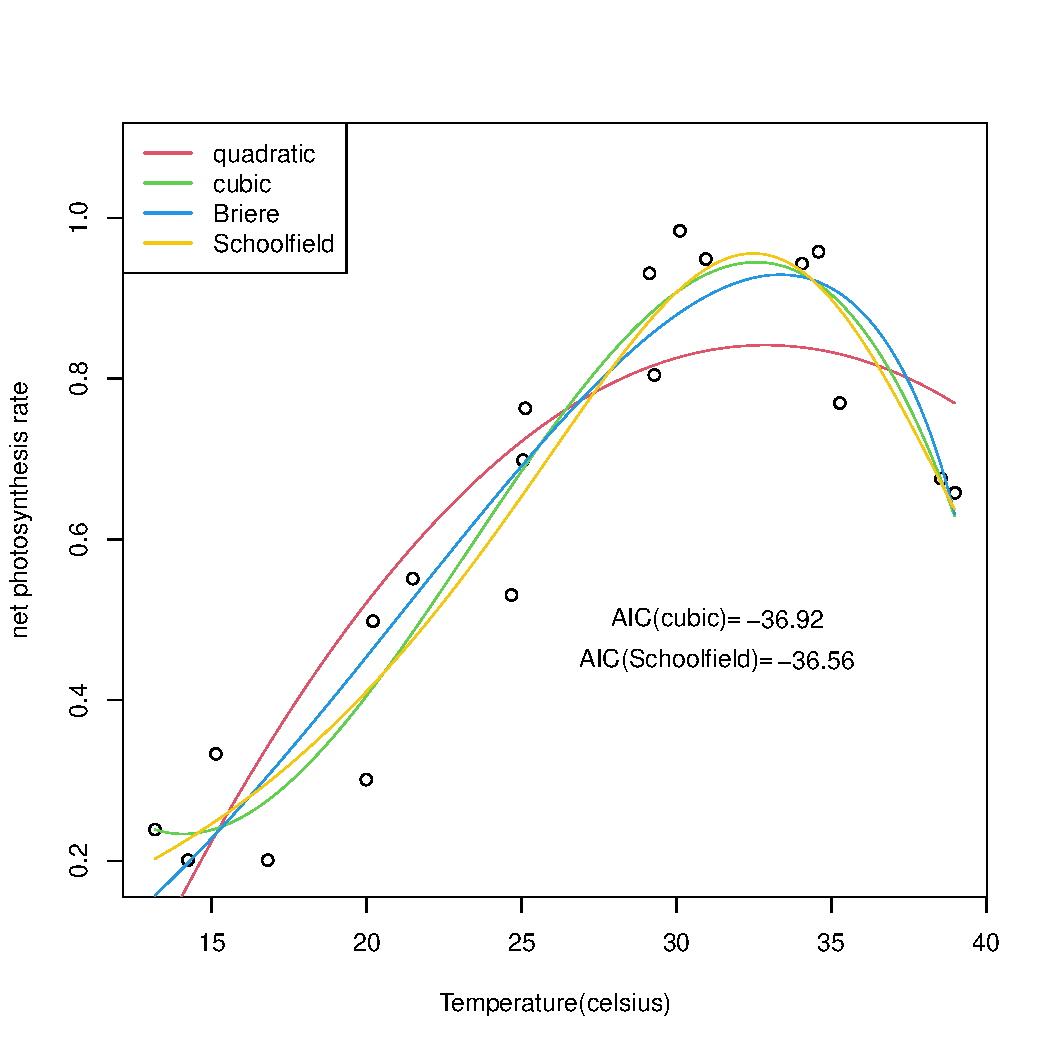
\includegraphics[scale=0.7]{../results/341.pdf}
    \caption{An example of all fitted models to a temperature response curve of net photosynthesis rate. Cubic (linear phenomenological) and Schoolfield (non-linear mechanistic) models are the better fits.}
    \label{fig:341}
\end{figure}

\begin{figure}[H]
    \centering
    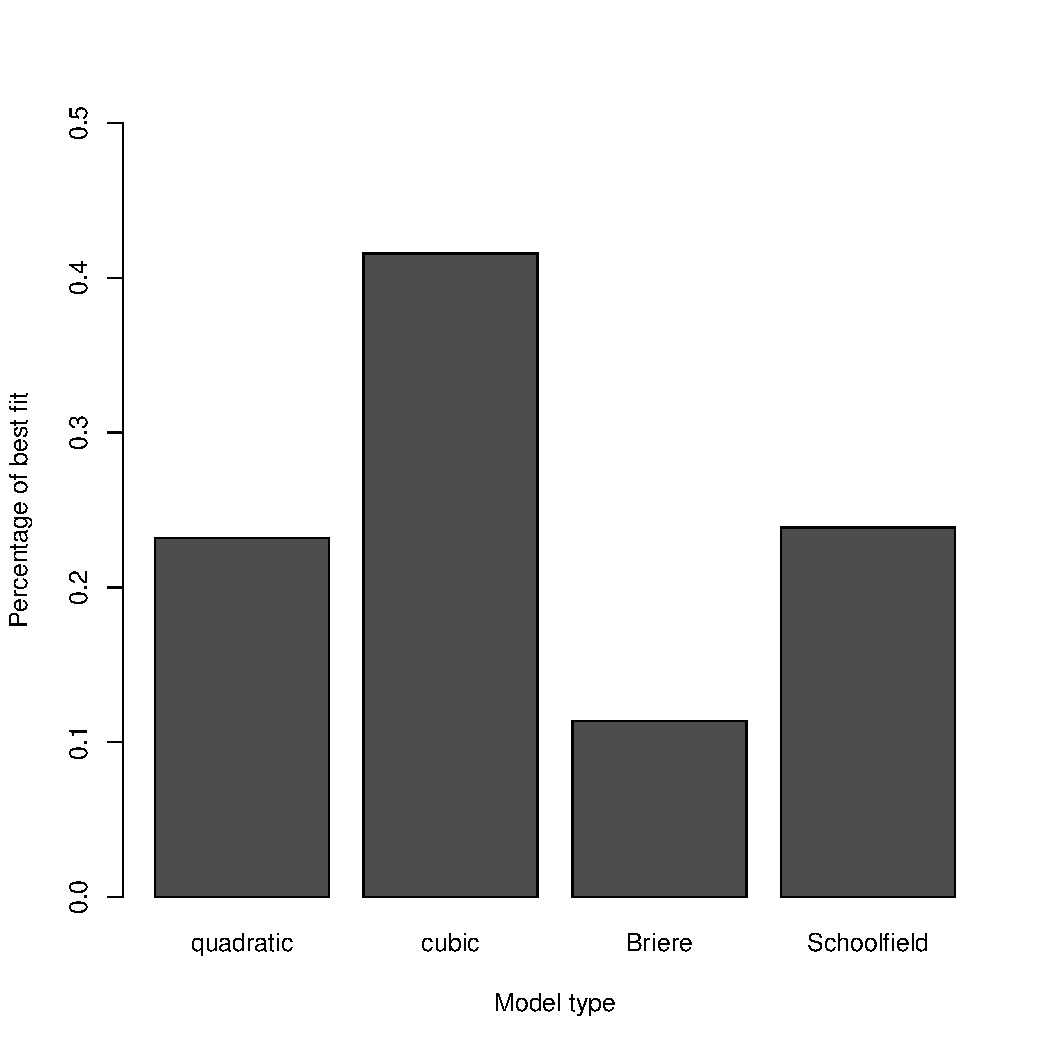
\includegraphics[scale=0.7]{../results/bestfit.pdf}
    \caption{Best fitted models selected based on AIC (left) and BIC (right).}
    \label{fig:bestfit}
\end{figure}

\begin{figure}[H]
    \centering
    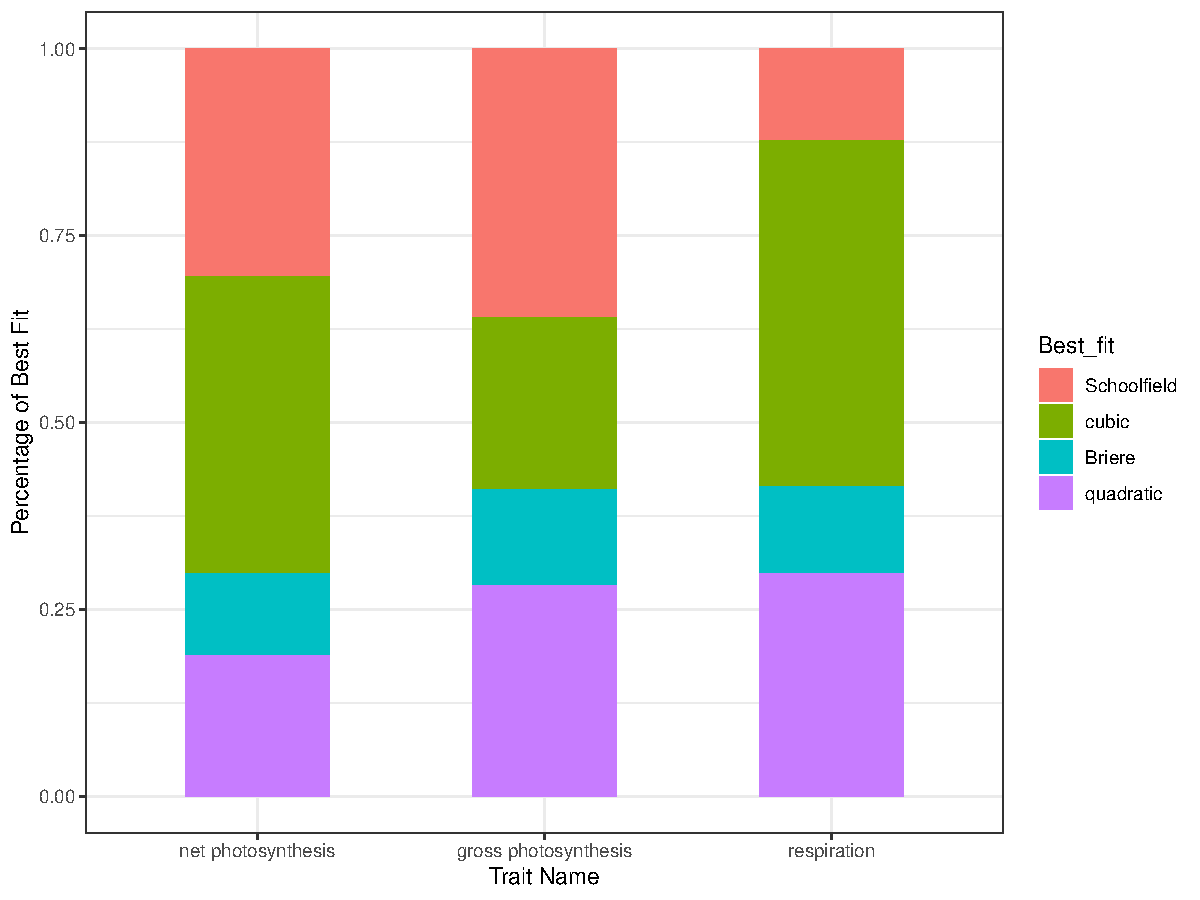
\includegraphics[scale=0.6]{../results/sub_trait.pdf}
    \caption{Best fitted models for respiration and photosynthesis, based on BIC selection.}
    \label{fig:sub_trait}
\end{figure}

\begin{figure}[H]
    \centering
    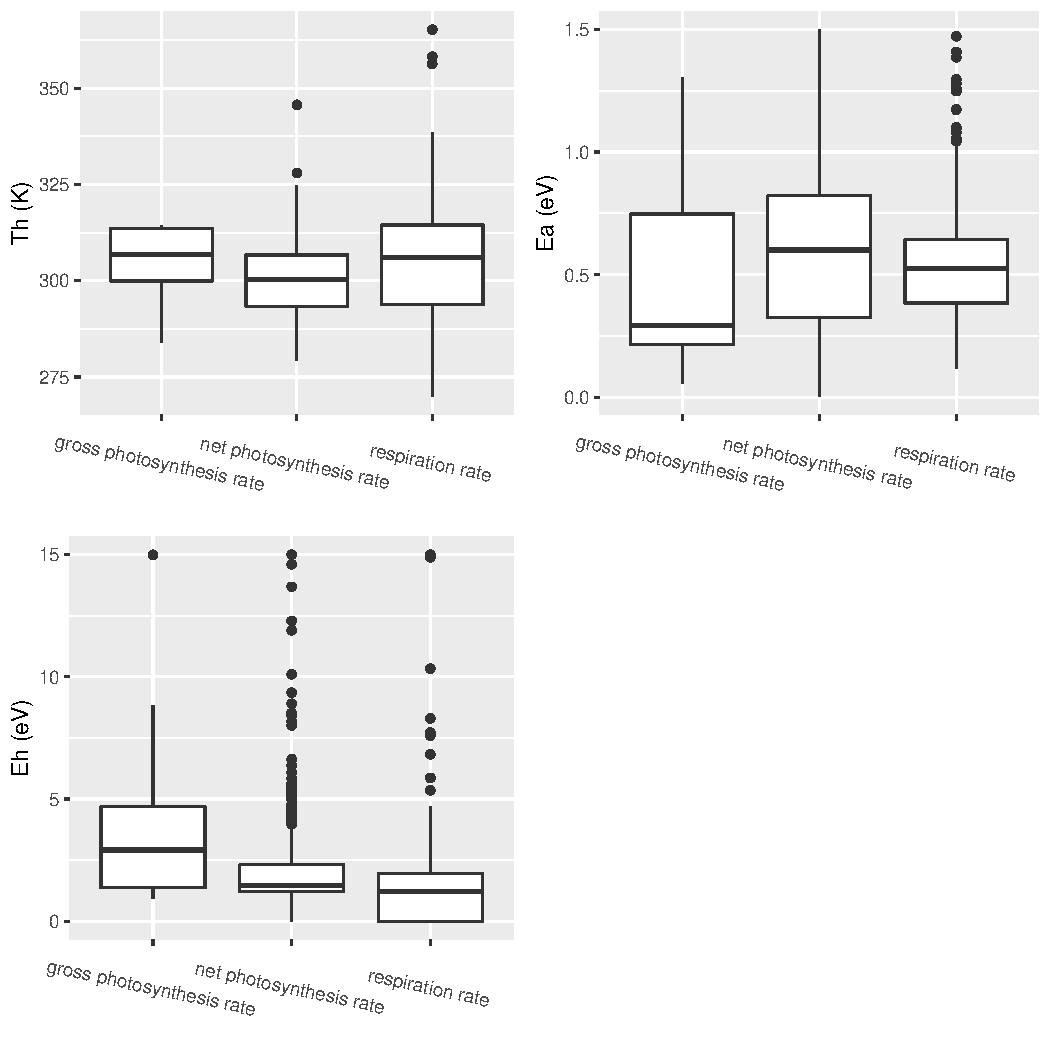
\includegraphics[scale=0.6]{../results/traits.pdf}
    \caption{Estimation of optimal temperature, activation and deactivation energy for respiration and photosynthesis by Schoolfield model. (x marking the mean values)}
    \label{fig:traits}
\end{figure}

\begin{figure}[H]
    \centering
    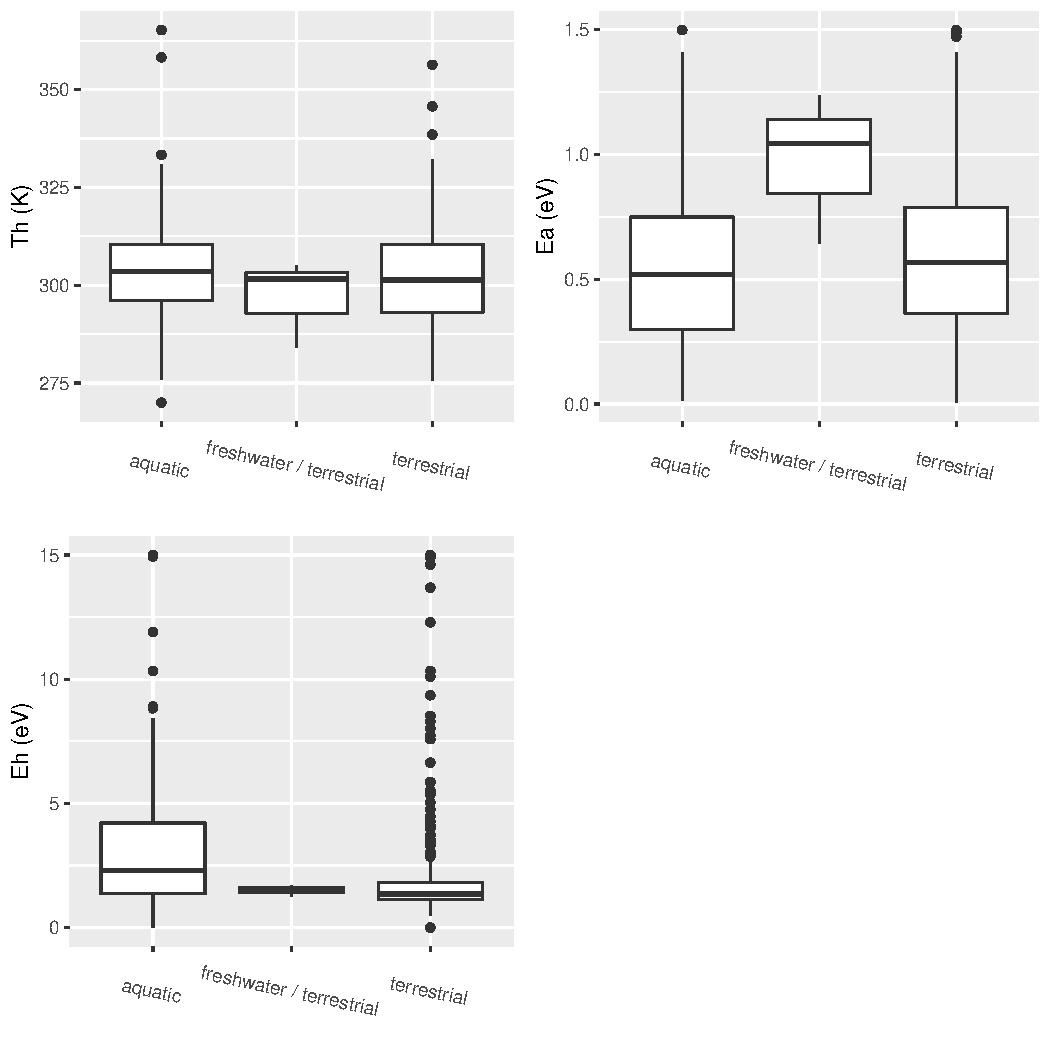
\includegraphics[scale=0.6]{../results/habitat.pdf}
    \caption{Estimation of optimal temperature, activation and deactivation energy for organisms from different habitats, by Schoolfield model. (x marking the mean values)}
    \label{fig:habitat}
\end{figure}

\section{Discussion}
%Start by reminding the reader about what the original goals of the study were
%State key findings succinctly
%Then discuss their implications in the wider context (with additional referencing beyond what you had in the intro).
%Include a paragraph or two of caveats/shortcomings with clear indication of what future work can do to address them.
%End with conclusion that delivers the final take-away messages.
In this project, I have fitted four models --- three phenomenological and one mechanistic to collected field data subset to compare and determine the suitability of these models to the data and look for patterns in the estimation made by the mechanistic Schoolfield model. 

The thermal performance curves normally show a similar shape that increases with temperature then rapidly decrease after reaching a maximum, this shape is usually resulted from a combination of thermodynamic effects of reaction rates and destabilization effects on intermolecular interactions by temperature \citep{schulte2011thermal}, so the non-linear models published all tend to describe a unimodal curve with a maximum trait value. 

The thermal response of respiration is better simulated by the linear models, since normal respiration activity does not require to be at optimum level, the denaturation temperature for respiration is recorded as approximately 40 $^{\circ}$C \citep{sage2007temperature}. However, most measurements conducted are around 20 $^{\circ}$C (at normal environmental temperature) for this study, which did not reach the deactivation temperature for respiration activity, resulting in a singularly increasing curve for respiration temperature responses. 

However, since temperature for optimum photosynthesis rate is much lower than respiration \citep{liu2018optimum}, the data collected for photosynthesis rate mostly contain values after the activation, generating the unimodal thermal curves. In this case, the non-linear models prevailed, especially the Schoolfield model. 

Comparing AIC and BIC selection method, a slight reduction of best fits was observed for the linear models in BIC. Since BIC method has a stronger punishment for model complexity; and by observing the original plots of data, unrealistic concave shapes, singularly falling data and completely messy datasets can be noticed, this could infer an overfitting of the linear models, especially the cubic. 

Not all parameter estimation results can be adapted for further analysation. The average temperature for maximum rate estimated for photosynthesis is approximately 25 $^{\circ}$C, though the estimations differ significantly between traits, this significance should not be taken into consideration for comparing due to the small temperature range of collected data. For the same reason, the deactivation energy should not be considered neither for respiration data,  but the activation energy for enzyme deactivation of photosynthesis was estimated as 2.5 eV in this project, lies within the suggested normal range of approximately 1.8 eV to 4.1 eV for enzyme reactions \cite{doran1995homogeneous}.

The activation energy can be adapted, however the average values of activation energy of respiration and photosynthesis estimated by the given data are higher than previously recorded values of approximately 0.65 eV and 0.3 eV \citep{allen2005linking, yvon2012reconciling}.

The general pattern for the estimation is that the activation energy and the maximum rate temperature of respiration is significantly higher than that of photosynthesis, that photosynthesis has higher temperature sensitivity, which is consistent with previous studies. And the average activation energy for aquatic organism overall metabolism is significantly higher than that for terrestrial organism, but the maximum rate temperature was not significantly different between these two habitats. 

Further work should include fitting more appropriate mechanistic models to for better predictions and understanding of the biological mechanisms, collecting data from a wider temperature range, and conducting further analysis to discover patterns of temperature response among different taxa or stages for this given data subset.  

Overall, the linear models (especially cubic) can provide better simulation for temperature response of respiration rates, however can result in slightly overfitting; and the Schoolfield model simulates better for the photosynthesis rates. The general pattern obtained from Schoolfield model estimation includes that respiration rate has higher temperature sensitivity than respiration, and the activation energy of aquatic organism overall metabolism is significantly higher than that for terrestrial organism. 

\bibliographystyle{agsm}
\bibliography{Miniproject_report}

\end{spacing}
\end{document}
